\section{Functional Analysis}
%Riesz theorem
%Banach-Alaoglu
Our preliminary goal in this section will be to show that $\M^1(X)$ is compact, provided that $X$ is a compact Hausdorff space. To show this we need some background in functional analysis, namely the Banach-Alaoglu and the Riesz-Representation Theorems, which are fundamental results from functional analysis.

\begin{theorem}[Banach-Alaoglu-Theorem,\cite{rudin:functional-analysis}]\label{thm:banach-alaoglu}
	Let $X$ be a topological (real) vector space and $V$ a neighborhood of $0$. Let 
	\[
	K:=\{\Lambda\in X^\prime\colon |\Lambda x|\leq 1 \forall x\in V\}
	\]
	then $K$ is weak*-compact.
\end{theorem}
%Note that the statement is still true if $X$ is a complex vector space. However, since we only need the statement for the real case, we will not discuss the complex version.

\begin{proof}
	Since $X$ is a topological vector space, there exists a number $0<\gamma(x)<\infty$ for every $x\in X$ such that $x\in \gamma(x)V$. %(In other words: every neighborhood of $0$ in a topological vector field is absorbing.) 
	Thus, for every $\Lambda\in X^\prime$ we have
	\[
	|\Lambda x|=|\gamma(x)\Lambda(\gamma^{-1}(x)\cdot x)|=\gamma(x)\cdot|\Lambda(\underset{\in V}{\underbrace{\gamma^{-1}(x)}\cdot x})\leq \gamma(x)\cdot 1=\gamma(x)
	\]
	Let $D_x:=[-\gamma(x),\gamma(x)]$ and define $P$ to be the cartesian product of all $D_x$ together with the product topology $\tau$. Since $D_x$ is compact for all $x\in X$, Tychonoff's theorem (\autoref{thm:tychonoff}) states that $P$ is compact as well. Since a function $f:X\to \R$ is determined by the relation $x\mapsto f(x)$, we can identify the elements of $P$ with functions $X\to \R$ with $|f(x)|\leq \gamma(x)$. (This identification works as follows: Let $z\in P$. The corresponding function $f_z:X\to\R$ is the function that maps every $x\in X$ to the $x$-coordinate of $z$.)
	
	With this identification, we see $K\subset X^\prime\cap P$. Therefore, $K$ inherits the weak* topology as a subspace of  $X^\prime$ and the subspace topology $\tau$ of $P$.
	\begin{myassertion}
		The described topologies coincide on $K$ and
	\end{myassertion}
	\begin{myassertion}
		The subset $K$ is a closed in $P$.
	\end{myassertion}

	It is clear that %this already implies that $K$ is weak*-compact as it is a closed subset of a compact space.
	once we proved this, the result of the theorem follows immediately since $K$ is a closed subset of a compact space and thus compact.
	
	Let $\Lambda_0\in K$ be fixed. Choose $\delta>0$ and $x_i\in X$ for all $1\leq i \leq n, n\in \N$. Now define
	\[
	W_1(n,(x_i)_{1\leq i\leq n},\delta):=\{\Lambda\in X^\ast\colon |\Lambda x_i-\Lambda_0 x_i|<\delta \text{ for } 1\leq i\leq n\}
	\]
	and
	\[
	W_2(n,(x_i)_{1\leq i\leq n},\delta):=\{f\in P\colon |f(x_i)-\Lambda_0 x_i|<\delta \text{ for } 1\leq i\leq n\}
	\]
	Then the collection of all $W_1$ form a local base for the weak*-topology of $X^\ast$ at $\Lambda_0$. Similarly the collection of all $W_2$ form a local base for the product topology $\tau$ of $P$ at $\Lambda_0$. Since $K\subset P\cap X^\ast$, we find
	\[
	W_1\cap K=W_2\cap K,
	\]
	hence the topologies coincide, as stated in Assertion 1.
	
	For the second assertion, let $f_0$ be an element in the $\tau$-closure of $K$. Choose $x,y\in X,\alpha,\beta\in \R, \epsilon>0$. The set of all functions satisfying $|f-f_0|<\epsilon$ at the points $x, y$ and $\alpha x+\beta y$ is a $\tau$-neighborhood of $f_0$, implying there exists an $f$ with that property in $K$. This $f$ is linear and thus,
	\begin{align*}
	f_0(\alpha x+\beta y)-\alpha f_0(x)+\beta f_0(y)=&f_0(\alpha x+\beta y)-\alpha f_0(x)+\beta f_0(y)\\
	&\qquad-\underset{=0}{\underbrace{f(\alpha x+\beta y)+\alpha f(x)+\beta f(y)}}\\
	&=(f_0-f)(\alpha x+\beta y)+\alpha (f-f_0)(x)+\beta (f-f_0)(y).
	\end{align*}
	Therefore,
	\begin{align*}
		|f_0(\alpha x+\beta y)-\alpha f_0(x)-\beta f_0(y)|<(1+|\alpha|+|\beta|)\epsilon.
	\end{align*}
	Since $\epsilon$ was arbitrary, we find that the expression above equals $0$, thus $f_0$ is linear.
	
	%check what is V
	Now, if $x\in V$ and $\epsilon >0$, it is analogous to show that $|f(x)-f_0(x)|<\epsilon$. Since $|f(x)|\leq 1$ by definition of $K$, we see that $|f_0(x)|\leq 1$. Thus $f_0\in K$. This shows that $K$ is closed in $P$.
\setcounter{assertion}{0}
\end{proof}

The following theorem is a standard result from functional analysis, providing a connection between measures and linear functionals. Note that this theorem holds for both the real and the complex case. However, since the real version is sufficient for our purposes, we will not consider the complex version.
\begin{theorem}[Riesz Representation Theorem, \cite{werner:funkana}]\label{thm:riesz}
	Let $X$ be a compact Hausdorff space. Then $C(X)^\ast$ is isometrically isomorph to $\M(X)$ with the mapping being given by
	\[
	T:\, M(X)\to C(X)^\ast,\quad (T\mu)(x)=\int_Xx\,\mathrm{d}\mu
	\]
\end{theorem}
\begin{proof}
	It is a well known result from measure theory that continuous functions are Borel measurable, thus the operator $T$ as above is well defined. Furthermore, the inequality \[
	\left|\int_X x\mathrm{d}\mu\right|\leq \int_X|x|\mathrm{d}|\mu|\leq \|x\|_\infty\|\mu\|.
	\]
	implies that $\|T\|\leq 1$.
	
	Firstly, we will show that $T$ is an isometry. Let $\mu\in\M(X)$. Consider the Hahn-Jordan decomposition of $\mu$, i.e. write $\mu=\mu_+ -\mu_-$ with positive measures $\mu_+ $ and $\mu_-$ and $X=E_+\cup E_-$ for disjoint Borel sets $E_+$ and $E_-$ such that for all Borel sets $F\supset E_+$ (resp. $E_-$) $\mu_-(F)=0$ (resp. $\mu_+(F)=0$). Since $\mu$ is regular, so are $\mu_+$ and $\mu_-$. Thus, for all $\varepsilon>0$ there exist compact sets $C_+\subset E_+$ and $C_-\subset E_-$ with
	\begin{align*}
		\mu(E_+)-\varepsilon&&\leq&&\mu(C_+)&&\leq&& \mu(E_+),\\
		\mu(E_-)+\varepsilon&&\geq&&\mu(C_-)&&\geq&& \mu(E_-).
	\end{align*}
	In particular, $C_-$ and $C_+$ are disjoint, since $E_-$ and $E_+$ are disjoint. This implies that the function
	\[
	y(t)=\begin{cases}
	1&\text{if }t\in C_+\\
	-1&\text{if } t\in C_-
	\end{cases}
	\]
	is continuous on $C_+\cup C_-$. The Tietze-Urysohn theorem (\autoref{thm:tietze-urysohn}) now implies, that there is an extension $x\in C(X)$ with $\|x\|_\infty=1$. %maybe rename function x?
	
	For this $x$ the following holds:
	\begin{align*}
		\left|\int_X x\mathrm{d}\mu\right|&=\left|\int_{C_+}\mathrm{d}\mu+\int_{C_-}(-1)\mathrm{d}\mu+\int_{X\setminus(C_+\cup C_-)}x~\mathrm{d}\mu\right|&\\
		&\geq \mu(C_+)-\mu(C_-)-\left|\int_{X\setminus(C_+\cup C_-)}x~\mathrm{d}\mu\right|&\text{(by reverse triangle-inequality)}\\
		&\geq \mu(E_+)-\varepsilon-\mu(E_-)-\varepsilon-|\mu|(X\setminus(C_+\cup C_-))&(\text{since } \|x\|_\infty=1)\\
		&=|\mu|(X)-2\varepsilon-(|\mu|(X)-|\mu|(C_+)-|\mu|(C_-))\\
		&=\mu(C_+)-\mu(C_-)-2\varepsilon&(\text{note } \mu(C_-)=-\mu_-(C_-))\\
		&\geq \mu(E_+)-\varepsilon-\mu(E_-)-\varepsilon-2\varepsilon\\
		&=|\mu|(X)-4\varepsilon.
	\end{align*}
	Thus, $\|T\mu\|\geq \|\mu\|-4\varepsilon$ for all $\varepsilon\geq 0$, hence $\|T\mu\|\geq\|\mu\|$. This concludes the proof of isometry since $\|T\mu\|\leq\|\mu\|$.
	
	We will now prove the surjectivity. Let $x^\prime\in C(X)^\prime$ be positive in the sense that if $x(t)\geq 0$ for all $t$, then $x^\prime(x)\geq 0$. We will now construct a regular Borel measure $\mu$ with $T\mu=x^\prime$. Note that we can't use $\mu(E)=x^\prime(\chi_E)$, since $\chi_E$ is not continuous in general. Instead, we proceed as follows: Let $O$ be a open subset of $X$ and define
	\[
	\mu^\ast(O)=\sup\{x^\prime(x)\colon 0\leq x\leq 1, \overline{\{t\colon x(t)\neq 0\}}\subset O \}
	\]
	and for arbitrary $E\subset X$
	\[
	\mu^\ast(E)=\inf\{\mu^\ast(O)\colon E\subset O, O \text{ open}\}.
	\]
	
	Now, we see that this $\mu^\ast$ is a outer measure, i.e. $\mu^\ast(E)\geq 0$ for all $E\subset X$, $\mu(\emptyset)=0$, $\mu^\ast(E)\leq \mu^\ast(F)$, if $E\subset F$ and $\mu^\ast\left(\bigcup_{n=1}^\infty E_n\right)\leq\sum_{n=1}^{\infty}\mu^\ast(E_n)$. For open sets $V$, we see 
	\begin{equation}\label{eq:riesz}
	\mu^\ast(V\cap F)+\mu^\ast(V^c\cap F)\leq \mu^\ast(F)\qquad \forall F\subset X
	\end{equation}
	
	Now, let $\Sigma_\mu:=\{V\subset X\colon V \text{ satisfies }\eqref{eq:riesz}\}$. The Extension Theorem of Carathéodory (\autoref{thm:measure-extension}) 
	then implies that $\Sigma_\mu$ is a $\sigma$-Algebra and $\mu^\ast\mid_{\Sigma_\mu}$ is a measure. By %$\eqref{eq:riesz}$ 
	construction all open sets are contained in $\Sigma_\mu$, we have $\Sigma\subset \Sigma_\mu$, thus $\mu:=\mu^\ast\mid_\Sigma$ is a regular (by construction), positive Borel measure and $x^\prime(x)=\int x\mathrm{d}\mu$ for all $x\in C(X)$.
	
	The general case for arbitrary $x^\prime\in C(X)^\prime$ can be reduced to the case of positive functionals. For $x\in C(X)$ define $x_+(t)=\max\{0,x(t)\}, x_-(t)=\max\{0,-x(t)\}$ and for $x\geq 0$ let
	\[
	x^\prime_+(x)=\sup\{x^\prime(y)\colon 0\leq y\leq x\}
	\]
	and for arbitrary $x\in C(X)$
	\[
	x^\prime_+(x)=x^\prime_+(x_+)-x^\prime_+(x_-).
	\]
	With this definition, $x^\prime_+$ is linear and continuous. Furthermore, $x^\prime_+(x)\geq 0$ in the sense mentioned above and $x^\prime_-:=x^\prime_+-x^\prime\geq 0$. We can apply essentially the same prove to $x^\prime_+$ and $x^\prime_-$ as we did to positive functionals and obtain positive regular Borel measures $\mu_+$ and $\mu_-$ with
	\[
	x^\prime(x)=x^\prime_+(x)-x^\prime_-(x)=\int_X x\mathrm{d}\mu_+-\int_Xx\mathrm{d}\mu_-\qquad \forall x\in C(X).
	\] 
	We can conclude that for $\mu=\mu_+-\mu_-$ we have $T\mu=x^\prime$.
	
	We now showed that $T$ is a isometry and surjective. This already implies that $T$ is a isometric isomorphism.
\end{proof}


We can now apply the previous two results to show the following theorem.
\begin{theorem}\label{thm:compactness}
	Let $X$ be a compact Hausdorff space. Then $\M^1(X)$ is weak*-compact.
\end{theorem}
\begin{proof}
	By Riesz-Representation-Theorem (\autoref{thm:riesz}), we can identify $\M(X)$ with $C(X)^\prime$. Clearly, $\M^1(X)$ is a closed subset of $\M(X)$ in the weak*-topology. Furthermore, $\M^1(X)$ is isometrically isomorph to the unit sphere in $C(X)^{\prime,+}$. The Banach-Alaoglu-Theorem (\autoref{thm:banach-alaoglu}) now states that the unit ball in $C(X)^\prime$ is weak*-compact and since closed subsets of compact sets are compact, the statement follows.
\end{proof}

%do I need the Schauder fixed point theorem at all now???
%\begin{theorem}[Schauder fixed-point theorem,\cite{werner:funkana}]
%	Let $C\neq\emptyset$ be compact and convex subset of a normed space and let $F: C\to C$ continuous. Then there is a $x\in C$ with $F(x)=x$.
%\end{theorem}
%
%\begin{proof}
%	Let $\epsilon>0$. Let $\tilde{\Gamma}$ be a covering of C consisting of $\epsilon$-balls. Since $C$ is compact there is a finite subcover $\Gamma=\{U_\epsilon(x_j)\}$ for some finite collection $\{x_j\}_{1\leq j\leq n}$, i.e.
%	\begin{equation*}\label{eq:covering}
%	C\subset \bigcup_{j=1}^n U_\epsilon(x_j)
%	\end{equation*}
%	
%	Let $\phi_j:C\to \R$ denote the continuous functions defined by
%	\[
%	\phi_j(x)=\begin{cases}
%	\epsilon-\|x-x_j\|& \text{ if } \|x-x_j\|<\epsilon\\
%	0&\text{ if }\|x-x_j\|\geq \epsilon
%	\end{cases}
%	\]
%	and define
%	\[
%	\phi: C\to \R, \quad \phi(x)=\sum_{j=1}^{n}\phi_j(x)
%	\]
%	Clearly, $\phi(x)>0$ for all $x\in C$. Therefore $\lambda_j:=\frac{\phi_j}{\phi}, j=1,\dots, n$ are well-defined continuous maps on $C$ with $0\leq \lambda_j(x)\leq 1$ and $\sum_{j=1}^{n}\lambda_j(x)=1$ for all $x\in C$.
%	
%	Let $E$ be the vector space spanned by the $x_i$ and $C^\prime=C\cap E$. Since there is only a finite number of $x_i$ the space $E$ has finite dimension and $C^\prime$ is a nonempty, compact, convex subset of $E$. We observe that the convex combination 
%	\[
%	\Phi(x)=\sum_{j=1}^{n}\lambda_j(x)x_j
%	\] 
%	is contained in $C^\prime$, hence $\Phi\circ F\mid_{C^\prime}\colon C^\prime\to C^\prime$ a continuous endofunction.
%	
%	With the Brouwer fixed-point theorem we conclude that $F$ has a fixed-point.%todo evtl etwas ausführlicher
%\end{proof}



%Schauderscher Fixpunktsatz für minimax theroem

For the remainder of this section we will consider critical points of spaces, which, in some sense, can be thought of as the \glqq corners\grqq{} of a topological space. We will also see the Theorem of Krein-Milman, which states that under certain conditions (see below) we can go back and forth between the actual topological space and its extreme points. We follow the discussion from \cite{werner:funkana} and finally apply this theory to show that measures with finite support are dense in $\M^1(X)$.

\begin{definition}
	Let $X$ be a vector space and $K\subset X$ convex.
	\begin{enumerate}
		\item A set $F\subset K$ is called a side of $K$, provided $F$ is convex and 
		\[
		x_1,x_2\in K, 0<\lambda<1,\lambda x_1+(1-\lambda)x_2\in F\Rightarrow x_1,x_2\in F
		\]
		\item A point $x\in K$ is said to be an extreme point of $K$, if $\{x\}$ is a side of $K$.
%		 provided \[
%	x_1,x_2\in K, 0<\lambda<1, \lambda x_1+(1-\lambda)x_2=x\Rightarrow x_1=x_2=x
%	\]
%	holds. 
We denote the set of extreme points of $K$ by $\mathrm{ex}K$
\end{enumerate}
\end{definition}

The following picture can be found in Werner \cite{werner:funkana} and illustrates above definition.

\begin{figure}[h]
\begin{centering}
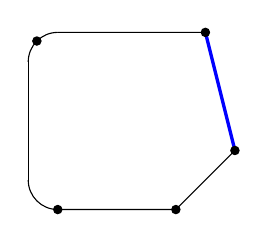
\begin{tikzpicture}[scale=0.75]
	\draw (0,0)--(2,0)--(3,1)--(2.5,3)--(0,3);
	\draw (-0.5,0.5) arc [start angle=180, end angle=270, radius=0.5];
	\draw (0,3) arc [start angle=90, end angle=180, radius=0.5];
	\draw (-0.5,0.5)--(-0.5,2.5);
	\draw[blue, very thick] (3,1)--(2.5,3);
	\filldraw (2,0) circle (2pt);
	\filldraw (0,0) circle (2pt);
	\filldraw (3,1) circle (2pt);
	\filldraw (2.5,3) circle (2pt);
	\filldraw (-0.3536,2.8536) circle (2pt);
\end{tikzpicture}
\caption{The points mark some extreme values. The blue line is a side.}
\end{centering}
\end{figure}

\begin{theorem}[Krein-Milman Theorem]\label{thm:krein-milman}
	Let $X$ be a locally convex, non-empty Hausdorff space and let $K\subset X$ be compact, convex and not empty.
	\begin{enumerate} 
		\item $\mathrm{ex}K\neq \emptyset$\label{krein-milman-1}.
		\item $K=\overline{\mathrm{conv}}\mathrm{ex}K$\label{krein-milman-2}.
	\end{enumerate}
\end{theorem}

\begin{proof}
	\begin{enumerate}
		\item Let $\mathcal{F}$ be the set of all  closed non-empty sides of $K$.  Since $K$ is itself a closed, non-empty side, we see that $\mathcal{F}\neq \emptyset$. Clearly, $\mathcal{F}$ is inductively ordered in terms of inclusion since the intersection of two closed sides is a closed side, which is nonempty since $K$ is compact\footnote{Recall the following: Let $(X,\mathcal{T})$ be a compact topological space. Then for any family of closed sets $(A_i)_{i\in I}$ in $(X,\mathcal{T})$ with $\bigcap_{i\in I}A_i=\emptyset$, then there exists a finite number of elements $i_1,\dots, i_n$ in $I$ with $\bigcap_{j=1}^n A_{i_j}=\emptyset$}. By the lemma of Zorn, there exists a minimal element $F_0$. Assume for a contradiction that $F_0$ does not consist of a single point. Applying the Hahn-Banach theorem (\autoref{thm:banach-separation}) yields the existence of points $x_0,y_0\in F_0, x^\prime\in X^\prime$ with
		\[
		\mathrm{Re}x^\prime(x_0)<\mathrm{Re}x^\prime(y_0).
		\]
		Now consider
		\[
		F_1=\left\{x\in F_0\colon \mathrm{Re}x^\prime(x)=\sup_{y\in F_0}\mathrm{Re}x^\prime(y)
		\right\}.
		\]
		Since $F_0$ is compact and $x^\prime$ continuous, $F_1\neq \emptyset$. Furthermore $F_1$ is closed and a side of $F_0$. Thus, $F_1$ is a side of $K$ as well, hence $F_1\in \mathcal{F}$. However, $x_0\not\in F_1$ implies $F_1\subsetneq F_0$. This contradicts the minimality of $F_0$.
		
		\item Let $K_1:=\overline{\mathrm{conv}}\mathrm{ex}K$. Then $K_1$ is compact, convex and not empty. Clearly $K_1\subset K$. Assume for a contradiction $K_1\neq K$. Then there exists $x_0\in K\setminus K_1$. By the Hahn-Banach Theorem (\autoref{thm:banach-separation}) there exists $x^\prime \in X^\prime, \varepsilon>0$ with
	\begin{equation}\label{eq:krein-milman}
	\mathrm{Re}x^\prime(x)\leq \mathrm{Re}x^\prime(x_0)-\varepsilon\quad \forall x\in K_1.
	\end{equation}
	Now let $F:=\{x\in K\colon \mathrm{Re}x^\prime(x)=\sup_{y\in X}\mathrm{Re}x^\prime(y)\}$. As before, we see that $F$ is a closed side of $K$ and not empty. By part \ref{krein-milman-1} we know that $\mathrm{ex}F\neq \emptyset$. Furthermore, $\mathrm{ex}F=\mathrm{ex}K\cap F\subset \mathrm{ex}K$. However \eqref{eq:krein-milman} implies 
	\[
	(\mathrm{ex}K)\cap F\subset K_1\cap F=\emptyset.
	\]
	This is a contradiction.\qedhere
\end{enumerate}
\end{proof}


We will now see an application of the Krein-Milman Theorem, which shows that measures can be approximated arbitrarily good by measures with finite support. The proof is partly due to Chad \cite{chad}.
\begin{theorem}\label{thm:finite-support}
	Let $X$ be a compact, non-empty Hausdorff space. Then the measures in $\M^1(X)$ with finite support form a dense subset of $\M^1(X)$.
\end{theorem}
\begin{proof}
	Firstly, note that $C(X)$ is a metric space with the metric that is induced by the variation norm, hence it is Hausdorff. This implies that the dual space $C(X)^\prime$ equipped with the weak*-topology is (completely) Hausdorff. Furthermore, it is clear that $C(X)^\prime$ is convex and therefore also locally convex. Now consider the subspace $K:=\{\phi\in C(X)^{\prime,+}\colon \|\phi\|=1\}$. Then $K$ is isometrically isomorph to $\M^1(X)$ by Riesz representation theorem and thus compact (see Banach-Alaoglu Theorem \ref{thm:banach-alaoglu}), convex and not empty.
	
	It is now sufficient to show that the extreme points of $\M^1(X)$ are given by $V:=\{\delta_x:x\in X\}$, where $\delta_x$ is the Dirac measure at point $x\in X$. (Note that the singletons are always Borel-measureable since $X$ is required to be Hausdorff.) 
	
	We begin by showing $V\subset \mathrm{ex}X$. Let $x\in X$ and $\mu,\nu\in \M^1(X)$ such that $\delta_x=\lambda \mu+(1-\lambda)$. Now, let $A\in \mathcal{B}(X)$. If $x\in A$, then by definition $\delta_x(A)=1$. Since $0\leq \mu,\nu\leq 1$ this implies $\mu(A)=\nu(A)=1$. If $x\not\in A$ then clearly $\delta_x(A)=0=\lambda\mu(A)+(1-\lambda)\nu(A)$ and thus $\nu(A)=\mu(A)=0$. In other words $\mu=\nu=\delta_x$.
	
	For the other inclusion, consider $\mu\in \M^1(X)\setminus V$. Since $X$ is a compact Hausdorff space, the support of $\mu$ is measurable and not empty. The support then has to include at least two points $x_1$ and $x_2$. Since $X$ is Hausdorff, there exists a open neighborhood $U$ of $x_1$ with $x_2\not\in U$. Since $U$ is open, it is Borel measurable. Then $0<\mu(U),\mu(X\setminus U)<1$. Now define measures $\nu,\lambda\in \M^1(X)$ as follows for $A\in \mathcal{B}(X)$:
	\[
	\nu(A)=\frac{1}{\mu(U)}\mu(A\cap U)\quad\text{ and }\quad \lambda(A)=\frac{1}{\mu(X\setminus U)}\mu(A\cap (X\setminus U)).
	\]
	Then for all $A\in \mathcal{B}(X)$,
	\begin{align*}
	\mu(A)&=\mu(A\cap U)+\mu(A\cap (X\setminus U))\\
	&=\mu(U)\cdot \nu(A)+(1-\mu(U))\cdot \lambda(A),
	\end{align*}
	thus $\mu$ is not a extreme point of $\M^1(X)$.
	
	With part \ref{krein-milman-2} of \autoref{thm:krein-milman} the statement follows.
\end{proof}